
\documentclass{article}
\usepackage[spanish]{babel} %Definir idioma español
\usepackage[utf8]{inputenc} %Codificacion utf-8
\usepackage{amssymb, amsmath, amsbsy, wasysym}
\usepackage{multirow} % para tablas
\usepackage{graphicx}
\usepackage{hyperref}
\usepackage{listings}
\usepackage[ruled, vlined, spanish, linesnumbered]{algorithm2e} %Para escribir algoritmos
\title{Proyecto de programación avanzada\\Calificación de películas}
\author{Emmanuel Peto Gutiérrez\\Rodrigo Fernando Velázquez Cruz}
\begin{document}
\maketitle

\section{Introducción}

Muchas veces queremos conocer información sobre lo que vamos a comprar o lo que vamos a ver (si se trata de una serie o película), para poder poder tomar una mejor decisión. En este proyecto se toma una tabla con información de calificaciones en diferentes películas y se filtran los resultados para mostrarlos en gráficas.

\subsection{Descripción del problema}

Los usuarios de servicios de streaming tienen problemas para seleccionar películas que le agraden y requieren una recomendación basado en lo que les ha gustado y lo que no les ha gustado. Se requieren conocer datos como la calificación promedio de películas, dadas ciertas restricciones (como el año de la película).

\subsection{Objetivo}

Diseñar un sistema que filtre información sobre las películas y sobre los datos de los usuarios que han calificado las películas. También, mostrar estadísticas en gráficas de barras sobre los resultados filtrados.

\section{El patrón Manager-Worker}

Este patrón de diseño también se le conoce como \textit{Master-Slave} o \textit{Map-Reduce}. Se utiliza para el procesamiento paralelo a través de múltiples procesos mediante un Manager y múltiples Workers.

is used for parallel processing. It follows a simple approach that allows applications to perform simultaneous processing across multiple machines or processes via a Master and multiple Workers.

A continuación se explicará cómo se utilizó este patrón de diseño paralelo en la realización del proyecto.

\subsection{La división de archivos}

Primero se divide el archivo principal en varios subarchivos de forma secuencial (i.e. por un solo hilo). El número total de subarchivos será igual a 4 veces el número de hilos disponibles en la CPU en la que se está ejecutando el programa, así que se tiene que calcular el número de hilos de forma dinámica.

\begin{center}
\includegraphics[scale=1]{division}
\end{center}

\subsection{La interpretación de la consulta}

El usuario dará una entrada de datos en los campos de texto que aparecen en la ventana para realizar la consulta. Se tiene que realizar un análisis sintáctico sobre la entrada. En la clase \texttt{Parser} se tienen métodos para interpretar la entrada del usuario y construir expresiones (objetos de la clase \texttt{Expresion}).

Una vez que se ha construído el conjunto de expresiones, se lanzan $n$ hilos (los trabajadores) y se envía la consulta ya interpretada a cada uno de ellos.

\begin{center}
\includegraphics[scale=1]{lanzar}
\end{center}

\subsection{El filtrado}

Cada hilo trabajador recibe las columnas a seleccionar y las condiciones de filtrado (las expresiones) desde su construcción. En el método \texttt{run} se realizan las operaciones de filtrado y selección, cada hilo leyendo de manera independiente sobre su propio subarchivo.

Cada vez que un hilo trabajador lee una línea, se verifica si cumple con las condiciones de filtrado, y si sí las cumple, escribe ese registro (borrando algunas columnas) en un archivo de salida. Todos los hilos escriben sobre el mismo archivo de salida, así que lo tienen que hacer de manera sincronizada para no colisionar.

\begin{center}
\includegraphics[scale=1]{filtrado}
\end{center}

\subsection{Las estadísticas}

Cuando ya se tiene el archivo filtrado, las clase \texttt{GeneraEstadisticas} se encargan de calcular estadísticas usando las calificaciones (columna \texttt{rating}) de las películas. Los datos estadísticos que se calculan son: promedio, mediana, mínimo y máximo.

Luego se muestran estas estadísticas en gráficas de barras mediante la clase \texttt{Main}.

\begin{center}
\includegraphics[scale=1]{estadisticas}
\end{center}

\section{La entrada y salida de datos}

En esta sección se explicará el formato en el que se deben ingresar los datos para que el programa funcione correctamente.

\subsection{Selección}

En el primer campo de texto (\texttt{TextField} de JavaFX) se deben ingresar las columnas a seleccionar separadas por comas. El parser sí hace una diferencia entre las mayúsculas y minúsculas, o sea que si se escribe ``TITLE'' no dará un resultado correcto porque la columna se llama ``title''. Las posibles columnas a seleccionar son:

\begin{itemize}
\item \textbf{idRating}: un número de 1 a $n$ que indexa las calificaciones.
\item \textbf{userId}: id del usuario.
\item \textbf{movieId}: id de la película.
\item \textbf{rating}: la calificación del 0 al 5 que un usuario específico le dio a una película específica.
\item \textbf{timestamp}: marca de tiempo en el que se realizó la calificación.
\item \textbf{title}: nombre de la película.
\item \textbf{year}: año en el que salió la película.
\item \textbf{genres}: géneros de la película (nótese que pueden ser más de uno).
\item \textbf{name}: nombre del usuario.
\item \textbf{lastname}: apellido del usuario.
\item \textbf{age}: edad del usuario.
\item \textbf{imdb}: url de una página que contiene más información sobre esa película.
\item \textbf{themoviedb}: lo mismo que la anterior pero de otra página.
\end{itemize}

Por ejemplo, si se quiere seleccionar \texttt{title, year, rating, genres} se deben escribir en el campo de texto que está debajo de la etiqueta \texttt{Indique las columnas a seleccionar.}

\includegraphics[width=\linewidth]{seleccion.png}

\subsection{Condición}

En el segundo campo de texto se deben escribir las condiciones de filtrado en forma normal disyuntiva. Primero se explicará cómo crear una expresión atómica.

Se dirá que una expresión atómica es cualquier expresión generada por la siguiente gramática:

Comparador := $< | > | <= | >= | = | <>$

Expr := variable Comparador valor

Donde una variable es el nombre de una columna y un valor es alguno de sus posibles valores en algún registro. Por ejemplo, se puede construir la expresión ``year = 1995'', lo que significa que se tomarán las películas que hayan salido en 1995.

Por supuesto, el usuario debería poder escribir más de una expresión atómica en su consulta. El sistema puede interpretar conjunciones (AND lógico) de expresiones atómicas, así que se pueden ingresar cadenas generadas con la siguiente gramática:

Conj := Expr $|$ Conj AND Conj

Por ejemplo, si se desea obtener todos los registros de películas que hayan sido calificadas por personas de entre 20 y 30 años, y que hayan salido después del 2000, se escribe la expresión:

age $>=$ 20 AND age $<=$ 30 AND year $>$ 2000

Las conjunciones después se pueden concatenar usando disyunciones (OR lógico). Estas cadenas se pueden generar con la siguiente gramática:

Disy := Conj $|$ Disy OR Disy

Si se requieren obtener los registros de todas las películas que hayan sido calificadas por personas de entre 20 y 30 años, para cualquier película que haya salido después del 2000, tal que su género sea Thriller u Horror se debe usar la siguiente expresión:

(age $>=$ 20 AND age $<=$ 30 AND year $>$ 2000 AND genres = Thriller) OR (age $>=$ 20 AND age $<=$ 30 AND year $>$ 2000 AND genres = Horror)

\includegraphics[width=\linewidth]{condicion}

\subsection{Gráficas de barras}

La salida de datos se escribe sobre un archivo de texto csv, pero también se muestran los datos en gráficas de barras en la ventana principal.

\includegraphics[width=\linewidth]{barras}

\section{Sobre la compilación y ejecución}

Debido a que usamos JavaFX para la interfaz, deben colocar los archivos .jar dentro del proyecto. A continuación se describen los pasos a realizar.

\begin{itemize}
\item[1.] Dirigirse a la página \url{https://openjfx.io/}
\item[2.] Dar click en el botón \textit{Download}, lo que lo enviará a la dirección \url{https://gluonhq.com/products/javafx/}
\item[3.] Descargar el SDK que sea adecuado para su sistema operativo y descomprimirlo.
\item[4.] Copiar todo lo que aparezca en la dirección \texttt{lib} de la carpeta de JavaFX y colocarlo en la dirección \texttt{MovieRec/lib} del proyecto.
\end{itemize}

Debido a que usamos un archivo \texttt{Makefile} para compilar y ejecutar el proyecto, requerirá tener instalado el comando \texttt{make}.

Para compilar y ejecutar debe colocarse en el directorio \texttt{MovieRec}, que es donde se encuentra el \texttt{Makefile} y escribir los siguientes comandos:
\begin{itemize}
\item Para compilar: \texttt{make compile}
\item Para ejecutar: \texttt{make run}
\end{itemize}

\end{document}


